\chapter{Discussion}

\section{Discrepancies in the Observed Redshifts of the Jets}
The redshifts of both jets in the short observation almost match to the predicted values - the redshift for the Eastern jet is slightly out of the error bar of predicted value (See the left part of Figure~\ref{redshift}).
Within the long observation, no significant redshifts change were observed for either jet. For the long observation, the predicted redshift value of the Western jet was -0.0097 and the predicted redshift value of the Eastern jet was 0.087. However, the average observed redshift values for the Western jet was 0.034, about 450\% larger than the predicted value. The difference being $\Delta z = 0.0437$ or 13110 km $\mathrm{s^{-1}}$. Since the discrepancy was already present at the beginning of the long observation, it is unclear when and how the redshift changed abnormally. Figure~\ref{redshift} shows the discrepancy between the observed and the predicted redshifts. The match between the predicted redshift and observed redshift of the Eastern jet indicate that two jets' behaviours were likely independent in the X-ray emitting region. This match to the conclusion drawn in \cite{Marshall2013}. According to Equation~\ref{relativistic_doppler}, the observed redshift depends on both the angle that the jet makes to the line of sight $\theta$, and on the velocity of the jet $v$. Therefore, the observed discrepancy indicates that the X-ray jet's velocities may have been affected by the environment which also perturbed the direction of the jet. 

According to Equation~\ref{relativistic_doppler}, if the redshift is 0.034, in order to make Western jet's speed to be 0.26c, $\theta$ needs to be 90.34\degree. If the redshift is -0.0097 as predicted, $\theta$ needs to be 99.69\degree. In order to have the jet have $\theta$ be the predicted value 99.69 \degree, the velocity needs to be 0.45c, which is almost twice of the accepted value, 0.26c. Figure~\ref{thetav} shows the relationship between $\theta$ and $v$, indicating that velocity perturbations alone are insufficient to explain the large Doppler shift change. Angular deviations of order 9\degree along the direction of precession would be needed to explain the discrepancy.

\begin{figure}
    \centering
    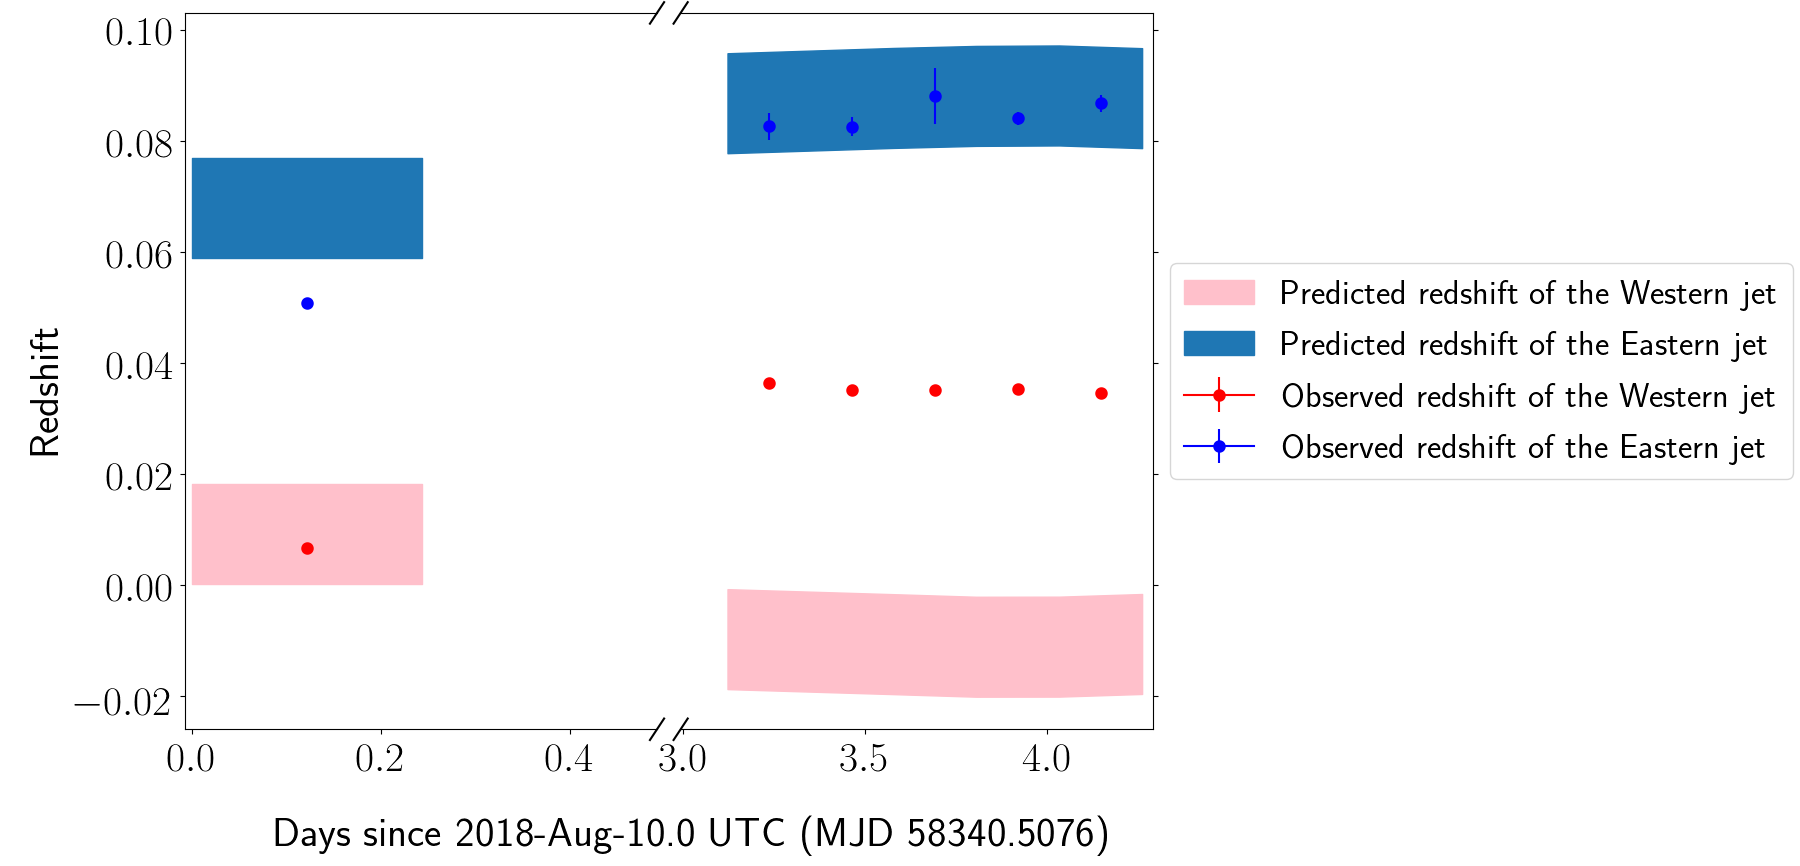
\includegraphics[width = \linewidth]{Chapters/Figures/redshiftv6.png}
    \caption{The observed redshifts from the 2018 observations with Chandra HETG and the predicted redshift according to the kinematic model. The blue and pink bands around the predicted redshift indicates the nutation motion of the jet.}
    \label{redshift}
\end{figure}


\begin{figure}[h!]
    \centering
    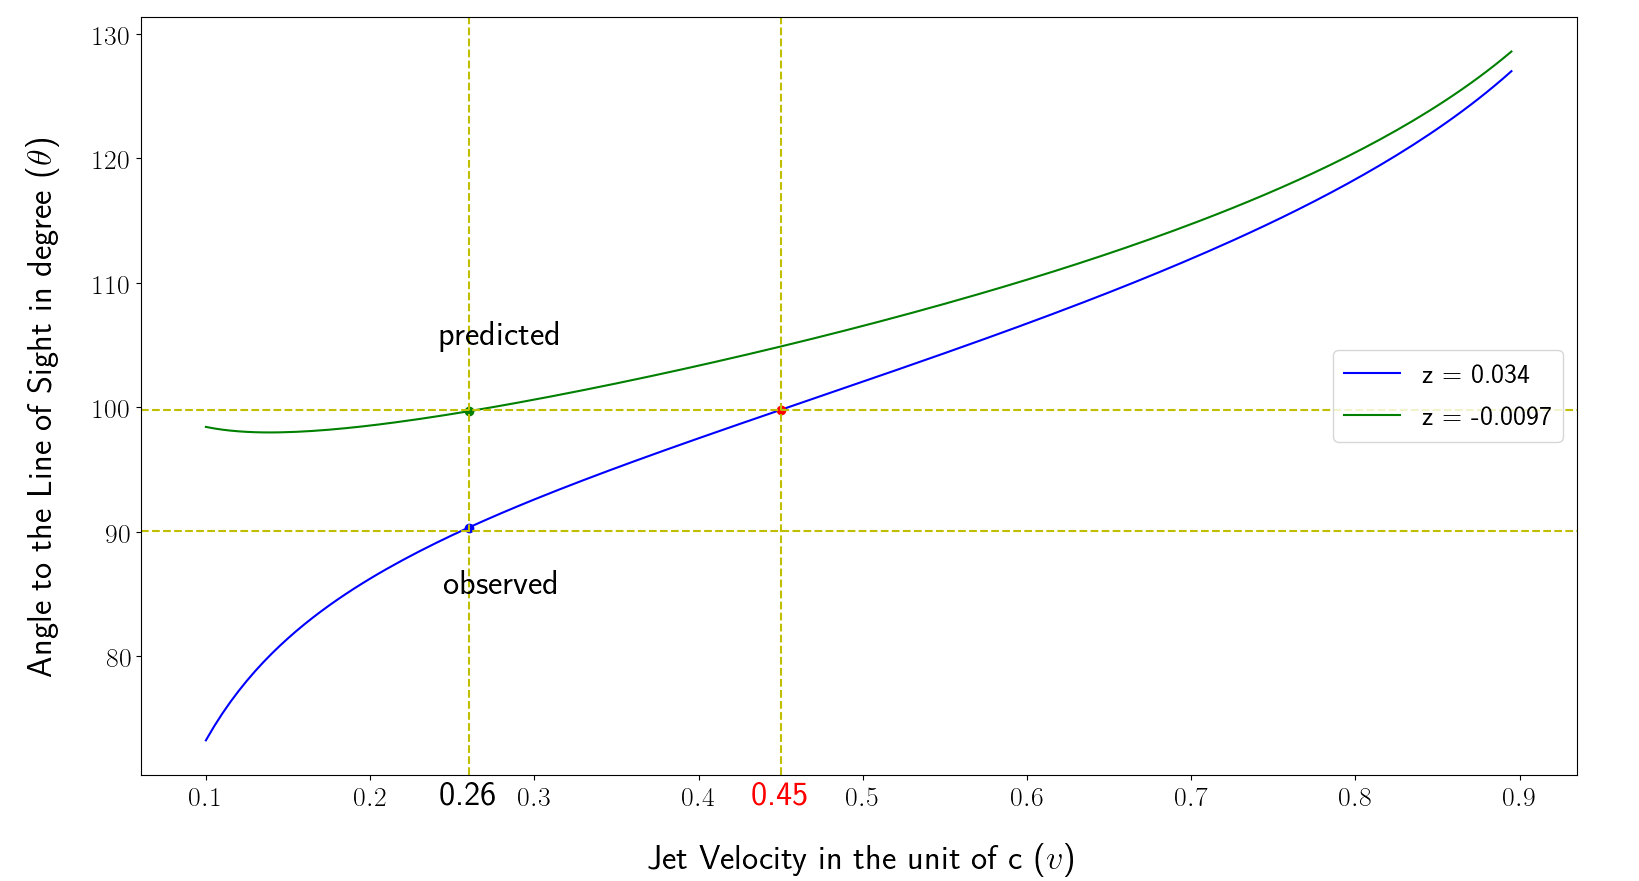
\includegraphics[width = \linewidth]{Chapters/Figures/thetav2.png}
    \caption{The relationship between $\theta$ and the velocity of the jet $v$ when the redshift value is 0.034 and -0.0097, respectively, from the 2018 observation. $\theta$ and $v$ }
    \label{thetav}
\end{figure}





\section{Line widths and Positions}
Table~\ref{tab:shortlinefluxes_west} - \ref{tab:longlinefluxes_east} show that the Doppler shifts of the lines in the Western and Eastern jet system are consistent with a single velocity to within the uncertainties for both the short and the long observation. The few deviations are mostly due to blended lines (e.g., line triplets) in each jet, and are not likely indicative of intrinsic variations. The lines responsible for largest deviations are mostly weak or blended, such as lines in the Eastern jet and the Si triplets. The line widths of the emission lines give information about Doppler broadening. Doppler broadening is the broadening of spectral lines due to the Doppler effect. The effect is caused by a distribution of velocities of atoms or molecules. Different velocities of the emitting particles contribute to different Doppler shifts. In plasma physics, the thermal Doppler broadening is one of the explanations to the broadening of a line. Thermal broadening is due to the thermal motion of the particles. The broadening depends only on the frequency of the spectral line, the mass of the emitting particles, and their temperature. Therefore, the broadening can be used for inferring the temperature of an emitting body. The velocity width of an emission line, or the mean speed of a particle can be found by 
\begin{equation}
    v = \dfrac{\sigma c}{\lambda_{obs}},
\end{equation}

where $\sigma$ is the width of the Gaussian. Line width measurements of the short observation for Western and Eastern jets are given in Table~\ref{linewidthshort_west} - \ref{linewidthshort_east}. Systematic errors due to poor continuum modeling, unresolved multiple blend lines modeled as single Gaussians, and unmodeled weak lines are estimated to be of order 100 - 150 km $\mathrm{s^{-1}}$ \citep{Marshall2013}. Although the statistic errors are not included, the line widths are measured in the wavelength 1.5 - 3.5 \AA\ are somewhat smaller than these found in previous papers \citep{Marshall2002, Lopez2006, Marshall2013}. The similarity of the line widths of all wavelengths range indicates that Fe {\sc xxv} is not significantly broader than other lines in the spectrum during the short observation.

\begin{deluxetable}{rc}
\tablecolumns{5}
\tablewidth{0pc}
\tabletypesize{\small}
\tablecaption{Western Jet Line Widths During the Short Observation
\label{linewidthshort_west} }
\tablehead{\colhead{Wavelength Range} &  \colhead{$v$}\\
  \colhead{(\AA)}  & \colhead{(km $\mathrm{s^{-1}}$)}& }
\startdata
1.5-3.5& 1028.2 \\
3.5-6.5& 1031.9 \\ 
6.5-10& 1036.3\\
\enddata
\end{deluxetable}


\begin{deluxetable}{rc}
\tablecolumns{5}
\tablewidth{0pc}
\tabletypesize{\small}
\tablecaption{Eastern Jet Line Widths
\label{linewidthshort_east} }
\tablehead{\colhead{Wavelength Range} &  \colhead{$v$}\\
  \colhead{(\AA)}  & \colhead{(km $\mathrm{s^{-1}}$)}& }
\startdata
1.5-3.5& 1347.6 \\
3.5-6.5& 1342.9 \\ 
6.5-10& 1340.7\\
\enddata
\end{deluxetable}



Since Eastern jet was faint during the long observation, line width measurements of only the long observation for Western jet are shown in Table~\ref{linewidthlong_west}. Line widths for different parts of the long observation were found separately. Comparing with the high-energy lines of the western jet in the short observation  (1028 km $\mathrm{s^{-1}}$, line widths of the western jet are significantly wider in the long observation (an average of 2146 km $\mathrm{s^{-1}}$). Within the long observation, lines in 1.5 - 3.5 \AA\ range are significantly broader than the lines in other ranges. Although Fe {\sc xxv} from the Western jet consists of unresolved lines, Fe {\sc xxvi} and Ni {\sc xxvii} (2100 km $\mathrm{s^{-1}}$) also dominate the broad line measurements in 1.5 - 3.5 \AA\ range. Ni is highly overabundant, as found in the plasma fitting in Chapter 4 (42.61 $\odot$ Ni for short observation and 30.21 $\odot$ Ni for the long observation). The line measurements in 6.5 - 10 \AA\ are somewhat larger than those reported in previous papers (729 $\pm$ 34 km $\mathrm{s^{-1}}$ \citep{Marshall2013}). More accurate values could be derived if more lines are fitted in longer wavelength range. 


\begin{deluxetable}{rccccc}
\tablecolumns{5}
\tablewidth{0pc}
\tabletypesize{\small}
\tablecaption{Western Jet Line Widths During the Long Observation
\label{linewidthlong_west} }
\tablehead{\colhead{} &  \colhead{Part \sc i}&  \colhead{Part \sc ii}&  \colhead{Part \sc iii}&  \colhead{Part \sc iv}&  \colhead{Part \sc v}\\ \colhead{Wavelength Range} &  \colhead{$v$}&  \colhead{$v$}&  \colhead{$v$}&  \colhead{$v$}&  \colhead{$v$}\\
  \colhead{(\AA)}  & \colhead{(km $\mathrm{s^{-1}}$)} & \colhead{(km $\mathrm{s^{-1}}$)}& \colhead{(km $\mathrm{s^{-1}}$)}& \colhead{(km $\mathrm{s^{-1}}$)}& \colhead{(km $\mathrm{s^{-1}}$)} }
\startdata
1.5 - 3.5&	15.7&	2245.3&	2213.3&	2042.2&	2232.4\\
3.5 - 6.5&	1064.1&	1082.8&	804.8&	984.2&	1293.9\\
6.5 - 10&	1120.8&	1136.2&	843.5&	1029.3&	1352.9\\

\enddata
\end{deluxetable}



\section{Jet Emission Line Fluxes}
Figure~\ref{west_flux} - \ref{east_flux} shows the line flux changes in the Western and Eastern jets, respectively. All the lines from the Western jet, including iron lines in the hardest energy region, appear on the spectrum with considerable line fluxes. The flux of Fe {\sc xxv} and Fe {\sc xxvi} from the Western jet did not decrease during the eclipse. Instead, these lines were significantly brighter than they were during the short observation 3 days ago. The changes of the fluxes of Fe {\sc xxv} and Fe {\sc xxvi} during the long observation did not show a regularly increasing or decreasing trend, indicating the fluctuations might be due to environmental activities instead of the eclipse. The increasing flux of and Si suggests that the cooler region of the Western jet was not occulted by the donor. This does not align with the model shown in Fig~\ref{geomtry_ss433} developed by \citep{Lopez2006}, where the outer region of the Western jet was blocked by the donor during the eclipse.\par 
In the Eastern jet, the flux of Fe {\sc xxv} goes to zero during the whole long observation. This suggests that the hard energy region of the Eastern jet was blocked by the donor. The blended lines of Fe {\sc xv} west and Fe {\sc xxvi} east made it harder to say whether the other Fe {\sc xxvi} from the Eastern jet was also blocked or not. Voigt profile modelling was able distinguish the two lines and fit two Gaussians in one region within a reasonable uncertainty. The flux of Fe {\sc xxvi} was not zero over the whole long observation. This questions the previous suggestion that the hard energy region of the jet was blocked since the temperature of the parts of the jet provide Fe {\sc xxvi} and Fe {\sc xxv} should not have a large difference, which means the region that emits Fe {\sc xxvi} and Fe {\sc xxv} should not be far part away. However, we have not yet been able to quantify this. Also, this observation does not agree with the conclusion by \citep{Marshall2013} that at most 20\% of the jet that provides the blue jet's Fe {\sc xxv} is blocked. The faintness of both hot and cool portions of the Eastern X-ray-emitting jet is unexpected because Eastern jet is usually the one that less blocked by the donor (see Figure~\ref{geomtry_ss433}).

\begin{figure}
    \centering
    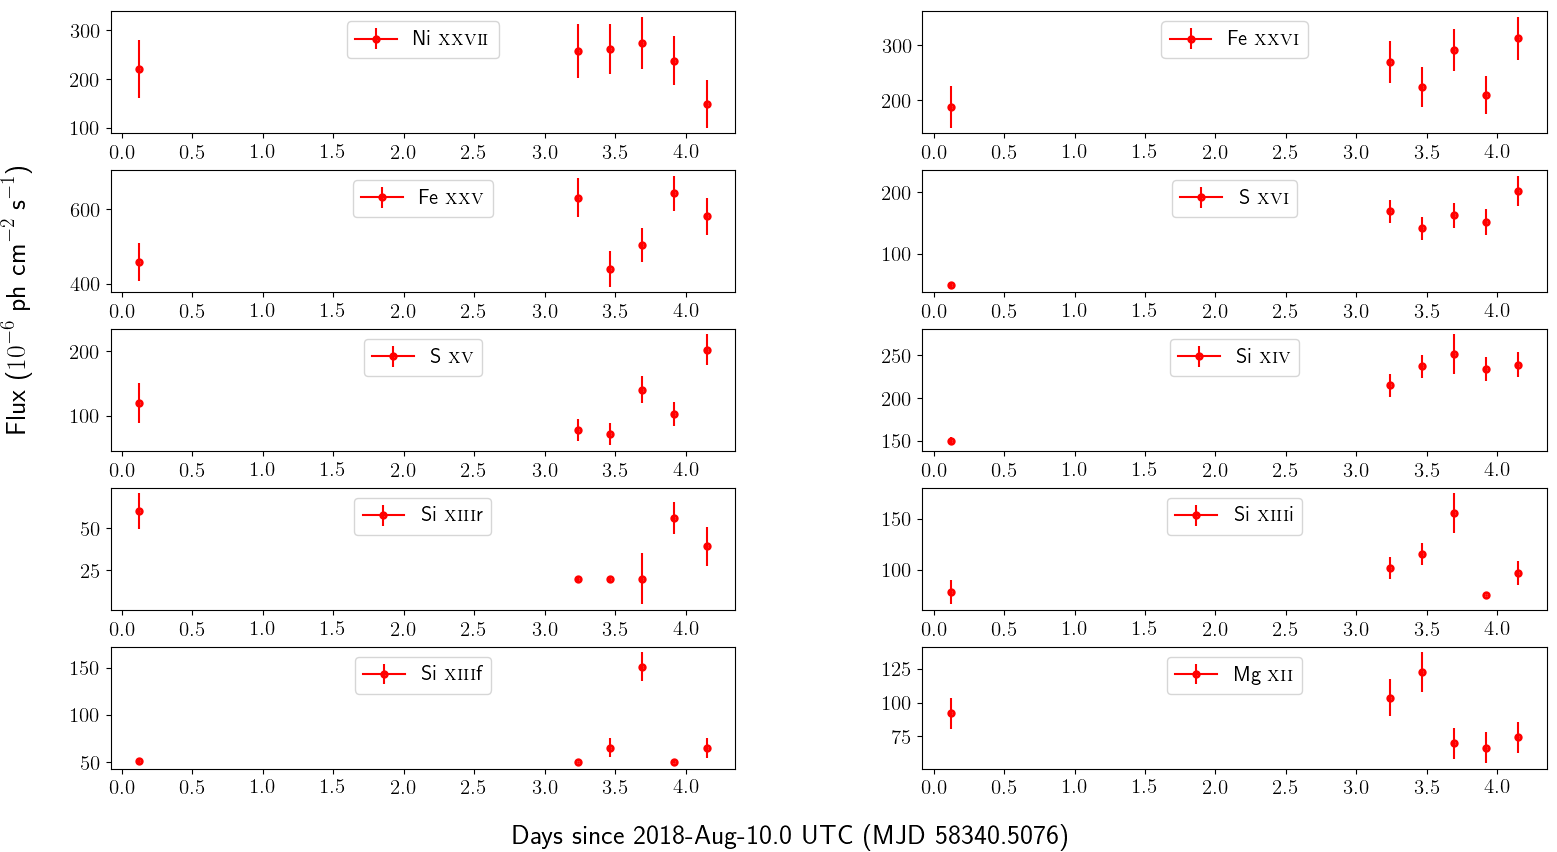
\includegraphics[width = \linewidth]{Chapters/Figures/west_flux.png}
    \caption{Flux changes of ten most prominent emission lines of the Western jet over the short and the long observation. The left most point is the line flux of certain element from the short observation while the four right most points are from the long observation. }
    \label{west_flux}
\end{figure}




\begin{figure}
    \centering
    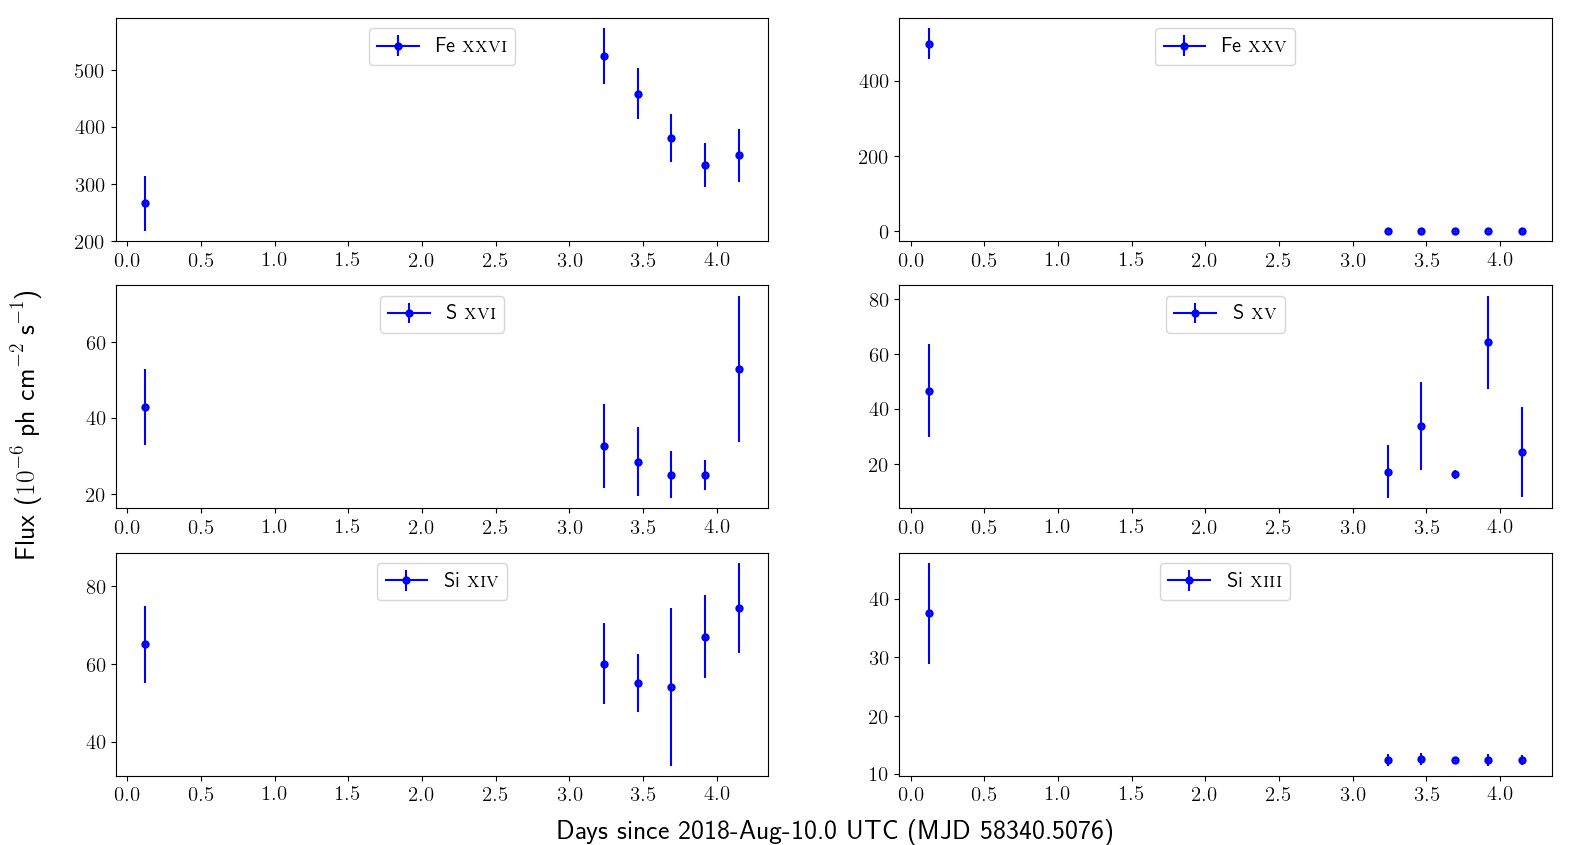
\includegraphics[width = \linewidth]{Chapters/Figures/east_flux.png}
    \caption{Same as Fig~\ref{west_flux}, but for the Eastern jet. The fluxes of Fe{\sc xxv} from the Eastern jet are zero over the long observation. S {\sc xv}, S {\sc xvi} and Si {\sc xiv} are faint and thus have larger uncertainties. Fe {\sc xxvi} east is blended with Fe {\sc xxv} west but with Voigt profile, it is able to fit two gaussians on one region moderately well.}
    \label{east_flux}
\end{figure}


\section{Power Law and Photon Index}

The predicted orbital phase of the end of the observation is 0.109. To verify whether the accretor came out of the eclipse at the end of our observation, we want to find the change of the normalization and the photon index of the spectra over the short and the long observation. Photon index is a measure of the dependence of radiative flux density on energy (or frequency). Normalization $K$ and photon index $\alpha$ satisfy the equation 
\begin{equation}
     N(E) = KE^{-\alpha}.
     \label{powerlaweq}
\end{equation}
After we take the log of Equation~\ref{powerlaweq}, we get 
\begin{equation}
     \mathrm{log}(N(E)) = \mathrm{log}(K) - \alpha \mathrm{log}(E).
     \label{powerlaweq}
\end{equation}
Figure~\ref{powerlaw} shows flux following a power law in energy. The cases when accretor is in the eclipse and out of the eclipse are shown in solid and dash lines.
\begin{figure}
    \centering
    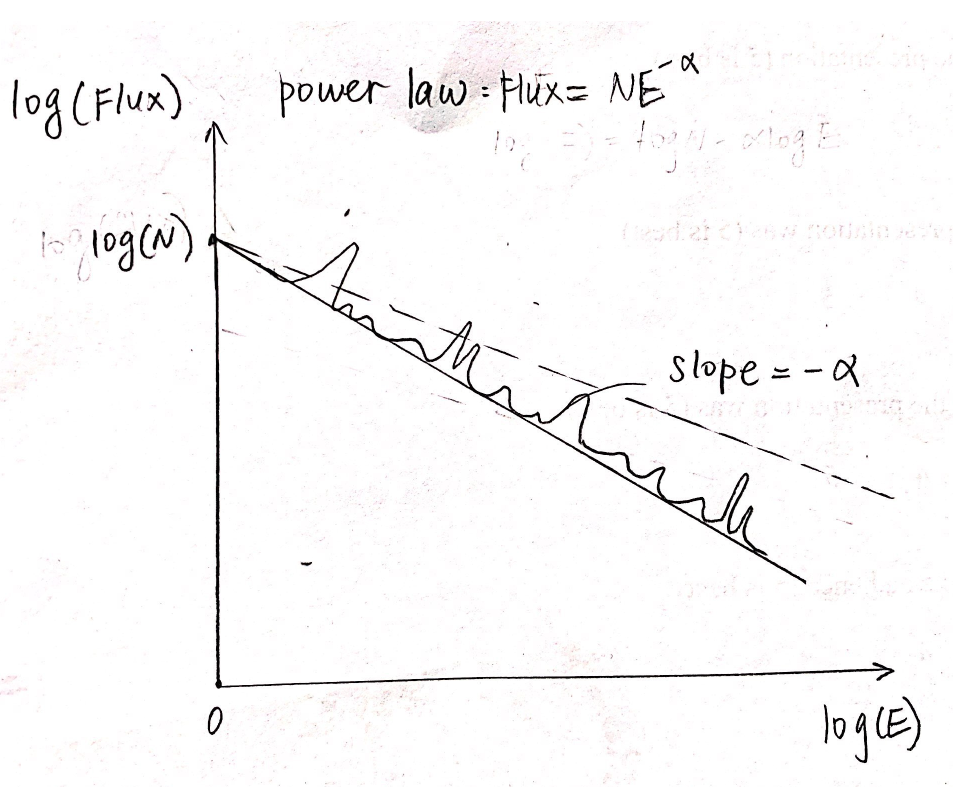
\includegraphics[scale = 0.4]{Chapters/Figures/powerlaw_v2.png}
    \caption{The log plot of power law that explains the relationship between the flux density and the energy. The solid line and the dash line show ideal scenarios when the accretor is in and out of the eclipse. The photon index decrease in this process. This is because the harder energy of the spectrum is more affected by the eclipse and thus when the source is coming out of the eclipse, the flux of the harder energy part will increase.}
    \label{powerlaw}
\end{figure}
Figure~\ref{power_law} show the change of normalization and photon index over time. There is a big jump in the normalizations and photon indices between the short observation and the first part of the long observation.  This might indicate some environmental activities in the low energy part of the jet before and during the long observation. The decreasing trend of photon index indicate that the high energy part of the jet is gradually coming out of the eclipse. Since the value of photon index at the end of the long observation is still 0.23 apart from the one at the short observation, it suggests that the accretor may not have totally come out of the eclipse, which can explain the disappearance of Fe {\sc xxv} of the Eastern jet at the end of the long observation. The reason for the decrease in normalization is uncertain. It is possible that the intrinsic accretion flow was changing during this time. 

\begin{figure}
    \centering
    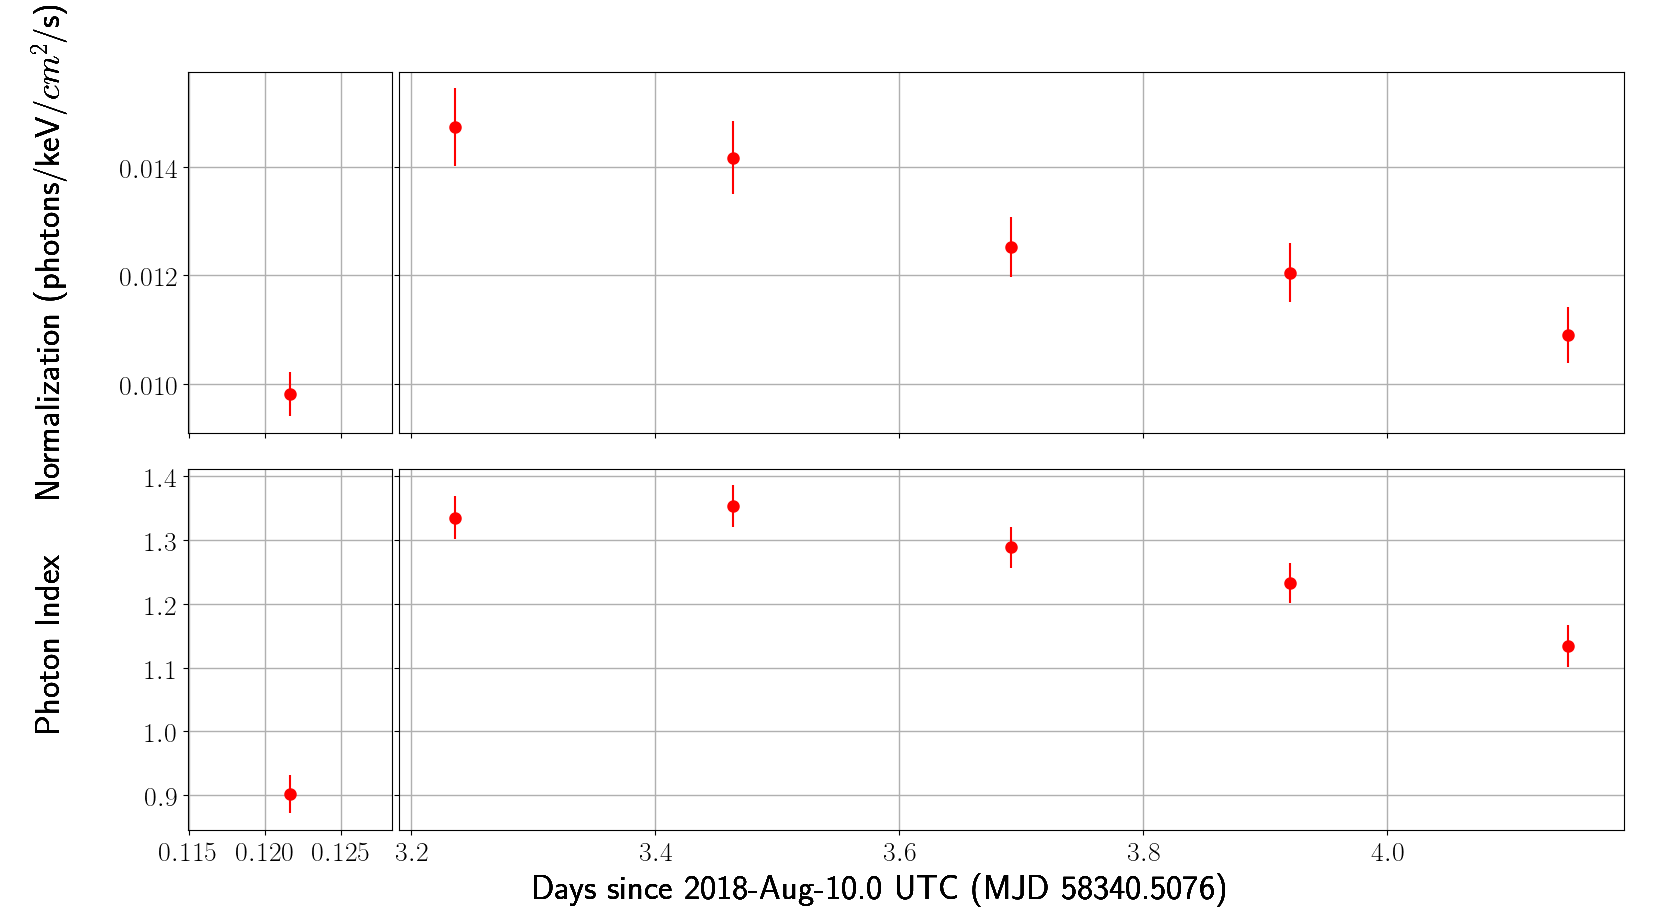
\includegraphics[width = \linewidth] {Chapters/Figures/powerlaw.png}
    \caption{The power law and photon index of the spectra over the short and the long observation}
    \label{power_law}
\end{figure}


